\documentclass{classrep}
\usepackage[utf8]{inputenc}
\frenchspacing

\usepackage{graphicx}
\usepackage[usenames,dvipsnames]{color}
\usepackage[hidelinks]{hyperref}
\usepackage{lmodern}
\usepackage{placeins}
\usepackage{url}
\usepackage{amsmath, amssymb, mathtools}
\usepackage{listings}
\usepackage{fancyhdr, lastpage}
\usepackage{amsfonts}

\pagestyle{fancyplain}
\fancyhf{}
\renewcommand{\headrulewidth}{0pt}
\cfoot{\thepage\ / \pageref*{LastPage}}

%--------------------------------------------------------------------------------------%
\studycycle{Applied Information Technology, 2 cycle}
\coursesemester{II}

\coursename{Soft Computing Laboratory}
\courseyear{2021/2022}

\courseteacher{dr inż. Kamil Stokfiszewski}
\coursegroup{Wednesday, 8:30}

\author{%
    \studentinfo[239671@edu.p.lodz.pl]{Jan Karwowski}{239671}\\
    \studentinfo[239676@edu.p.lodz.pl]{Kamil Kowalewski}{239676}\\
}

\title{Assignment 4.: Simple Genetic Algorithm}

\begin{document}
    \maketitle
    \thispagestyle{fancyplain}

    \tableofcontents
    \newpage

    \section{Main goal} \label{main_goal} {
        The main goal of this task is to prepare implementation of Simple Genetic
        Algorithm (SGA). The algorithm have to optimize function shown below:
        \begin{equation}
            f(x)=(e^x sin(10 \pi x)+1)/x+5
        \end{equation}
        on the $[0.5, 2.5] \subset \mathbb{R}$. This function is presented on fig.
        \ref{fig:fitness_function}.

        \begin{figure}[!htbp]
            \centering
            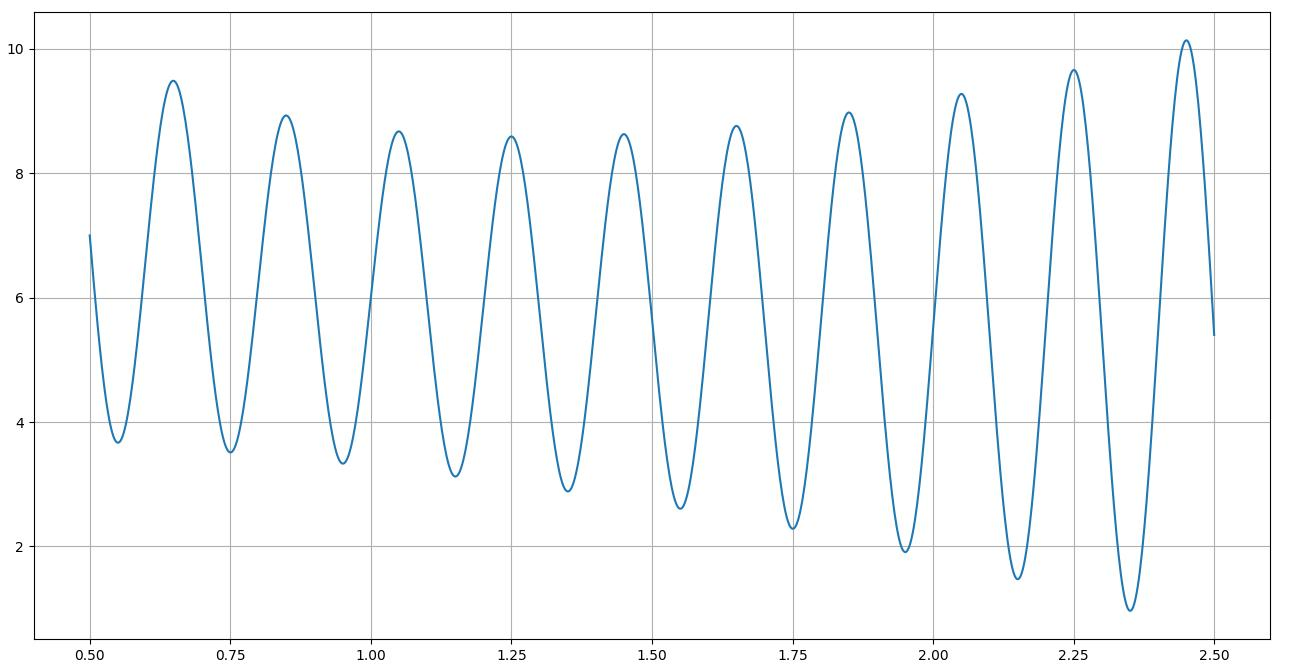
\includegraphics[width=0.95\textwidth]{img/fitness_function.jpg}
            \caption{Fitness function}
            \label{fig:fitness_function}
        \end{figure}
        \FloatBarrier
    }

    \section{Theoretical background} \label{theory} {
        Simple Genetic Algorithm (SGA) is a very basic and first implementation of genetic
        algorithm, which a general concept of algorithm based on the law of natural selection. It
        was created to find optimal solution of very compound problems, i.e. optimize complicated,
        multimodal functions of many variables. Since this particular version of genetic algorithm
        is ,,standardized'', there is no need to introduce more details. It should be enough to
        mark, that our implementation is possibly consistent with the original one. Any
        changes and variations are described below.
    }

    \section{Implementation} \label{implementation} {
        SGA was implemented in Python programming language, using common \emph{numpy} library.
        Fitness function and optimization range are hardcoded and taken from the task description.
        Program accepts 5 parameters:
        \begin{enumerate}
            \item solution accuracy as integer number of decimal digits (p)
            \item number of populations - number of SGA iterations (N)
            \item population size (M)
            \item crossover probability (pc)
            \item mutation probability (pm)
        \end{enumerate}

        The main function starts from computing required number of bits, necessary to encode all
        possible solutions with given accuracy and range. This number should be lower then $64$ -
        the max possible integer size. In fact, all the solutions are stored as $64$-bits integer
        values and all genetic operators are implemented using bitwise operators.
    }

    \section{Experiments and results} \label{results} {
        Two series of experiments were conducted. The first one explores impact of particular
        parameters on SGA's solution finding ability. In scope of this series for each set of
        parameters algorithm was run $50$ times and successful runs were counted. When the best
        solution's fitness from the very last population is greater then $10$ (see fig.
        \ref{fig:fitness_function}, then such a run is marked as successful, i.e. SGA found global
        optimum of the fitness function. Results of this series are presented in table
        \ref{tab:series_1_results}.

        \begin{table}[!htbp]
            \centering
            \caption{Results of first series of experiments}
            \begin{tabular}{|c|c|c|c|c|c|c|}
                \hline
                # & p & N & M & pc & pm & successful runs \\ \hline
                1 & 3 & 100 & 50 & 0.5 & 0.2 & 24 \\
                2 & 3 & 100 & 80 & 0.5 & 0.2 & 25 \\
                3 & 3 & 100 & 200 & 0.5 & 0.2 & 36 \\
                4 & 3 & 200 & 50 & 0.5 & 0.2 & 23 \\
                5 & 3 & 30 & 50 & 0.5 & 0.2 & 23 \\
                6 & 5 & 100 & 50 & 0.5 & 0.2 & 16 \\
                7 & 3 & 100 & 50 & 0.7 & 0.2 & 19 \\
                8 & 3 & 100 & 50 & 0 & 1 & 30 \\
                9 & 3 & 100 & 50 & 0 & 1 & 17 \\
                10 & 3 & 100 & 50 & 0.9 & 0.05 & 24 \\ \hline
            \end{tabular}
            \label{tab:series_1_results}
        \end{table}
        \FloatBarrier

        The second series of experiments explores SGA's behaviours during single run. Two
        experiments/runs was conducted and each of them is presented on a single chart, which
        presents best solutions' fitness (vertical axis) for next populations/iterations (horizontal
        axis) - fig. \ref{fig:low_mutation_probability} and \ref{fig:high_mutation_probability}.

        \begin{figure}[!htbp]
            \centering
            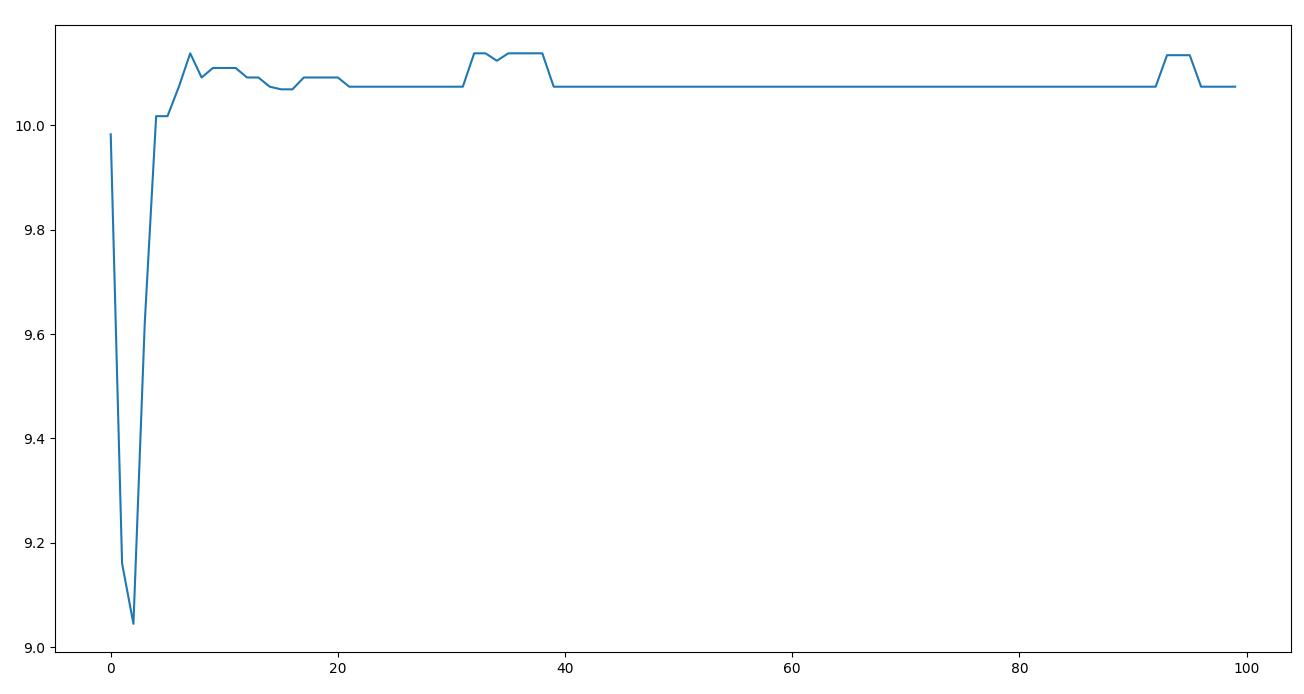
\includegraphics[width=1.1\textwidth]{img/low_mutation_probability.jpg}
            \caption{Low mutation probability}
            \label{fig:low_mutation_probability}
        \end{figure}

        \begin{figure}[!htbp]
            \centering
            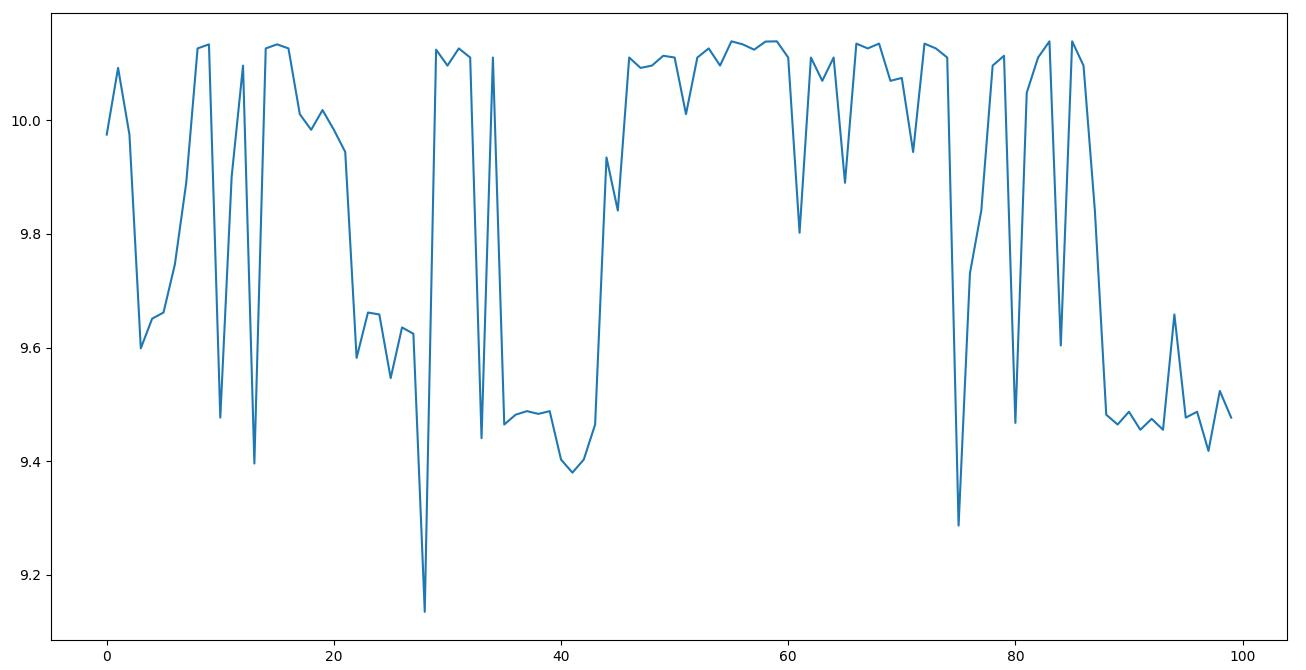
\includegraphics[width=1.1\textwidth]{img/high_mutation_probability.jpg}
            \caption{High mutation probability}
            \label{fig:high_mutation_probability}
        \end{figure}
        \FloatBarrier
    }

    \section{Summary and conclusions} \label{summary} {
        In table \ref{tab:series_1_results} we can see results of experiments, where impact of
        particular parameters on SGA behaviour was explored. The very first conclusion, or rather a
        \emph{remark}, is that these results are not very representative and should NOT be
        considered as important argument, when selecting best SGA hyperparameters. This is caused by
        strong stochastic nature of this algorithm, especially in context of this particular problem
        (fitness function). I.e. there is no strict rules, when this algorithm is able to find
        global optimum. On the other hand some observations can be made.

        First of all, when population size increase, then SGA can easier find global optimum. We can
        see it in rows 2. and 3. in compare to row 1., which is a reference. Another conclusion is,
        that changing number of iterations (number of populations) is not very important. This
        conclusion is related to this particular problem, and may be not very general. But in fact,
        in row 4. and 5. we can see no special difference, when compared to row 1. It could be
        caused by the fact, that this problem (fitness function) is relatively simple and global
        optimum may be found in the on of the first iterations. In row 6. required accuracy was
        increased and it noticeably degradates SGA - it seems to be intuitive behaviour. In the last
        rows (7, 8, 9, 10) probabilities of crossover and mutation was changed. We noticed that
        changing these values may have positive and negative impact as well, completely
        randomly in most cases.

        It is worth mentioning, that increasing mutation probability make searching process less
        stable, and it can produce completely different results, sometimes very good and sometimes
        very bad - it's just a random search. When mutation probability is greater, then searching
        process is more stable, it used to stay in good solutions, when it find some of them. We can
        see it in the results of second series of experiments in fig.
        \ref{fig:low_mutation_probability} and fig. \ref{fig:high_mutation_probability}.
    } 

    \begin{thebibliography}{0}
        % @formatter:off
        \bibitem{instruction}{Labolatory instruction, URL: https://ftims.edu.p.lodz.pl/pluginfile.php/75442/\\mod\_resource/content/1/soft\_comp\_lab\_04\_SGA.pdf}
        % @formatter:on
    \end{thebibliography}

\end{document}
